\documentclass{article}
\usepackage[margin=1in]{geometry}
\usepackage{amsmath,amsthm,amssymb}
\usepackage{bbm,enumerate,mathtools}
\usepackage{tikz,pgfplots}
\usepackage{chessboard}
\usepackage[hidelinks]{hyperref}
\usepackage{multicol} % Problem 35

\newenvironment{question}{\begin{trivlist}\item[\textbf{Question.}]}{\end{trivlist}}
\newenvironment{note}{\begin{trivlist}\item[\textbf{Note.}]}{\end{trivlist}}
\newenvironment{references}{\begin{trivlist}\item[\textbf{References.}]}{\end{trivlist}}
\newenvironment{related}{\begin{trivlist}\item[\textbf{Related.}]\end{trivlist}\begin{enumerate}}{\end{enumerate}}


\begin{document}
\rating{3}{2}
Given two vector valued functions
$u, v\colon \mathbb{R}^n \rightarrow \mathbb{R}^n$, that are linearly
independent at every point, let
$f\colon \mathbb{R}^n \times \mathbb{R}^n \rightarrow \mathbb{R}$ be
defined by \[
  f(x_0, x_1) = |\alpha| + |\beta| \text{ where }
  x_1 - x_0 = \alpha \cdot u(x_0) + \beta \cdot v(x_0).
\]
Next let the length of a curve $\Gamma\colon [0, 1] \rightarrow \mathbb{R}^n$
be given by \[
  \mathcal{L}(\Gamma) = \lim_{N \rightarrow \infty} \sum_{k = 0}^{N - 1} f\left(
    \Gamma\left(\frac{j}{N}\right), \Gamma\left(\frac{j + 1}{N}\right)
  \right).
\]
Let the distance $d: \mathbb{R}^n \times \mathbb{R}^n \rightarrow \mathbb{R}$
from $x_0$ to $x_1$ be given by the infimum of the length over all curves from
$x_0$ to $x_1$: \[
  d(x_0, x_1) = \inf\{\,\mathcal{L}(\Gamma): \Gamma(0) = x_0 \text{ and } \Gamma(1) = x_1\,\}.
\]
\begin{figure}[ht!]
  \centering
  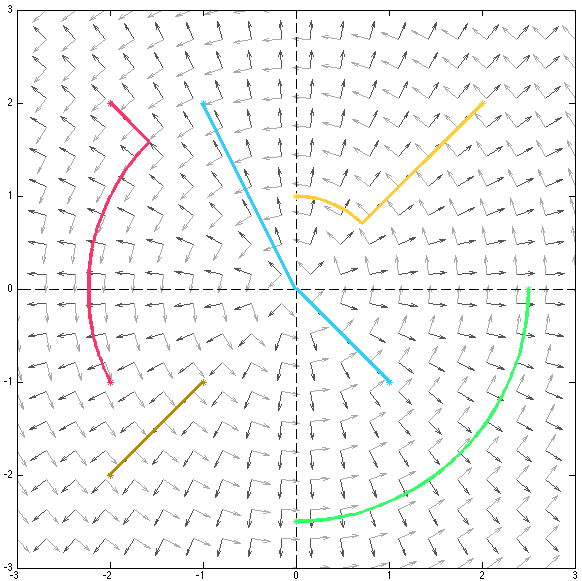
\includegraphics[width=100mm]{assets/Problem58_figure.png}
  \caption{
    Five examples of shortest curves when
    $u(x_1, x_2) = (x_1, x_2)/||(x_1, x_2)||$ and
    $v(x_1, x_2) = (-x_2, x_1)/||(x_1, x_2)||$.
  }
\end{figure}
\begin{question}
  What are the necessary conditions on $u$ and $v$ for this to be a well-defined
  metric space?
\end{question}
\begin{related}
  \item If $|u(x)| = |v(x)| = 1$ for all $x \in \mathbb{R}^n$, what is greatest
    possible (Euclidean) length of the circumference of a unit circle?
  \item If $u$ and $v$ are well-behaved and selected at random according to some
    distribution, what is the expected length of the circumference of a unit
    circle?
\end{related}
\end{document}
